\documentclass[12pt]{article}

\usepackage[utf8]{inputenc}
\usepackage{datetime}
\usepackage{amsthm}
\usepackage{amsmath}
\usepackage{amssymb}
\usepackage{enumitem}
\usepackage[english]{babel}
\usepackage{matlab-prettifier}
\usepackage{graphicx}
\usepackage[makeroom]{cancel}
\usepackage{afterpage}
\usepackage{capt-of}
\usepackage{bm}
\usepackage{float}

\DeclareMathOperator*{\argmin}{arg\,min}
\DeclareMathOperator*{\argmax}{arg\,max}

\newcommand\independent{\protect\mathpalette{\protect\independenT}{\perp}}
\def\independenT#1#2{\mathrel{\rlap{$#1#2$}\mkern2mu{#1#2}}}

\newtheoremstyle{colon}{\topsep}{\topsep}{}{}{\bfseries}{:}{ }{}
\theoremstyle{colon}
\newtheorem{exercise}{Exercise}
\newtheorem*{answer}{Answer}

\title{APC 523: Numerical Algorithms for Scientific Computing \\ Homework 2}
\author{Zachary Hervieux-Moore}

\newdate{date}{20}{04}{2019}
\date{\displaydate{date}}

\begin{document}

\maketitle

\clearpage

\begin{exercise}
  \textbf{"Barycentric" interpoloation formula}
\end{exercise}

\begin{answer}
  \begin{enumerate}[label=\alph*)]
    \item Recall the definitions:
      \begin{gather*}
        L_j(x) = \prod_{\substack{k = 0 \\ k \neq j}}^N \frac{x - x_k}{x_j - x_k} \\
        p_N(x) = \sum_{j=0}^N f_j L_j(x)
      \end{gather*}

      Suppose we are interpolating $f(x) = 1$, then our interpolating function $p_N(x) = 1$ and all $f_j = 1$ and thus we have
      \begin{gather*}
        p_N(x) = \sum_{j=0}^N f_j L_j(x) = \sum_{j=0}^N L_j(x) = 1
      \end{gather*}

    \item Substituting their definitions, we get,
      \begin{gather*}
        \frac{w_j^{(N)}}{x-x_j} \cdot L^{(N)}(x) = \frac{\prod_{\substack{k = 0 \\ k \neq j}}^N \frac{1}{x_j - x_k}}{x - x_j} \cdot \prod_{k=0}^N (x - x_k) \\
        = \prod_{\substack{k = 0 \\ k \neq j}} \frac{1}{x_j - x_k} \cdot \prod_{\substack{k = 0 \\ k \neq j}} x - x_k \\
        = \prod_{\substack{k = 0 \\ k \neq j}} \frac{x - x_k}{x_j - x_k} = L_j(x)
      \end{gather*}

      Now, taking the definition, we have
      \begin{gather*}
        L_j(x_j) = \prod_{\substack{k = 0 \\ k \neq j}}^N \frac{x_j - x_k}{x_j - x_k} = 1
      \end{gather*}

      Thus, $L_j(x_j)=1$ and we have $L_k(x_j) = 0$ for $k \neq j$  since $L^{(N)}(x_j)/(x-x_j) = 0$. Thus, the logical branch is
      \begin{gather*}
        L_j(x) = \begin{cases}
          \frac{w_j^{(N)}}{x-x_j} \cdot L^{(N)}(x), \text{ if } x \neq x_j \\
          1, \text{ o.w.}
        \end{cases}
      \end{gather*}

    \item Now, suppose $x = x_k$ for some $k$, then we have
      \begin{gather*}
        p_N(x_k) = \sum_{j=0}^N f_j L_j(x) = \sum_{j=0}^N f_j L_j(x_k) = f_k
      \end{gather*}

      Thus, we get that $p_N(x)$ can be rewritten as when substituing b) as
      \begin{gather*}
        p_N(x) = \begin{cases}
          L^{(N)}(x) \sum_{j=0}^N \frac{w_j^{(N)}}{x-x_j} f_j, \quad x \neq x_0, \mathellipsis, x_N \\
          f_k, \quad x = x_k
        \end{cases}
      \end{gather*}

    \item Using our results
      \begin{gather*}
        \sum_{j=0}^N L_j(x) = 1 \\
        L_j(x) = \frac{w_j^{(N)}}{x-x_j} \cdot L^{(N)}(x)
      \end{gather*}

      then,
      \begin{gather*}
        \sum_{j=0}^N \frac{w_j^{(N)}}{x-x_j} \cdot L^{(N)}(x) = 1 \\
        \implies L^{(N)}(x) \sum_{j=0}^N \frac{w_j^{(N)}}{x-x_j} = 1
      \end{gather*}

      Now, injecting this into the denominator of part c) yields,
      \begin{gather*}
        p_N(x) = \begin{cases}
          \frac{L^{(N)}(x) \sum_{j=0}^N \frac{w_j^{(N)}}{x-x_j} f_j}{L^{(N)}(x) \sum_{j=0}^N \frac{w_j^{(N)}}{x-x_j}}, \quad x \neq x_0, \mathellipsis, x_N \\
          f_k, \quad x = x_k
        \end{cases} \\
        \implies p_N(x) = \begin{cases}
          \frac{\sum_{j=0}^N \frac{w_j^{(N)}}{x-x_j} f_j}{\sum_{j=0}^N \frac{w_j^{(N)}}{x-x_j}}, \quad x \neq x_0, \mathellipsis, x_N \\
          f_k, \quad x = x_k
        \end{cases}
      \end{gather*}

    \item See the implementation in \texttt{question1.ipynb}

    \item See the implementation in \texttt{question1.ipynb}

  \end{enumerate}
\end{answer}

\clearpage

\begin{exercise}
  \textbf{Chebyshev nodes of the second kind}
\end{exercise}

\begin{answer}
  \begin{enumerate}[label=\alph*)]

    \item See the implementation in \texttt{question2.ipynb}

    \item See the implementation in \texttt{question2.ipynb}

    \item See the implementation in \texttt{question2.ipynb}

      \begin{enumerate}[label=\roman*)]
        \item The maximum relative errors are listed below
          \begin{center}
            \begin{tabular}{ c | c }
              Nodes & Relative error \\
              \hline
              4 & 1.58662e-2 \\
              8 & 1.62741e-6 \\
              16 & 1.03328e-13 \\
            \end{tabular}
          \end{center}

        \item The maximum relative errors are listed below
          \begin{center}
            \begin{tabular}{ c | c }
              Nodes & Relative error \\
              \hline
              4 & 1.25691 \\
              8 & 3.67927 \\
              16 & 51.0769 \\
            \end{tabular}
          \end{center}

        \item The maximum relative errors are listed below for the $1^{st}$ kind
          \begin{center}
            \begin{tabular}{ c | c }
              Nodes & Relative error \\
              \hline
              4 & 1.21570e-2 \\
              8 & 4.84377e-7 \\
              16 & 8.07804e-16 \\
            \end{tabular}
          \end{center}

          The maximum relative errors are listed below for the $2^{nd}$ kind
          \begin{center}
            \begin{tabular}{ c | c }
              Nodes & Relative error \\
              \hline
              4 & 1.17164e-2 \\
              8 & 5.27579e-7 \\
              16 & 1.02670e-15 \\
            \end{tabular}
          \end{center}

        \item The maximum relative errors are listed below for the $1^{st}$ kind
          \begin{center}
            \begin{tabular}{ c | c }
              Nodes & Relative error \\
              \hline
              4 & 7.50300e-1 \\
              8 & 3.91740e-1 \\
              16 & 8.31070e-2 \\
            \end{tabular}
          \end{center}

          The maximum relative errors are listed below for the $2^{nd}$ kind
          \begin{center}
            \begin{tabular}{ c | c }
              Nodes & Relative error \\
              \hline
              4 & 8.28912e-1 \\
              8 & 4.59605e-1 \\
              16 & 9.93219e-2 \\
            \end{tabular}
          \end{center}

      \end{enumerate}

    \item See the implementation in \texttt{question2.ipynb}.

      \begin{enumerate}[label=\roman*)]
        \item See the plots below. The slopes match the expected $\kappa$ as $N$ gets large enough.
          \begin{figure}[H]
            \centering
              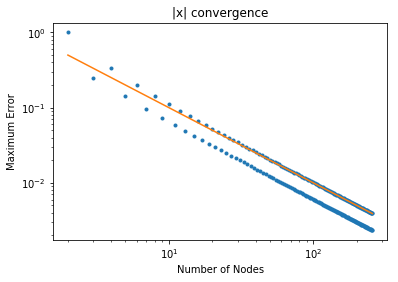
\includegraphics[width=0.8\textwidth]{q2dia.png}
            \caption{Convergence of $f(x) = \lvert x \rvert$}
          \end{figure}

          \begin{figure}[H]
            \centering
              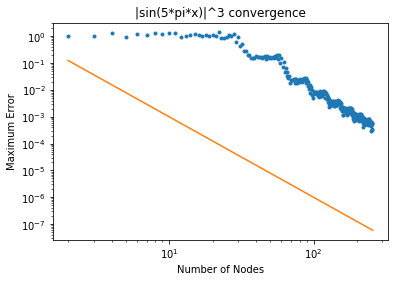
\includegraphics[width=0.8\textwidth]{q2dib.png}
            \caption{Convergence of $f(x) = \lvert \sin(5 \pi x) \rvert^3$}
          \end{figure}

          \begin{figure}[H]
            \centering
              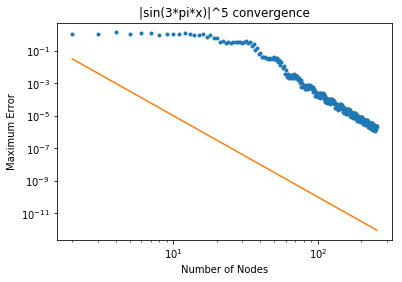
\includegraphics[width=0.8\textwidth]{q2dic.png}
            \caption{Convergence of $f(x) = \lvert \sin(3 \pi x) \rvert^5$}
          \end{figure}

        \item See the plots below. The slopes are linear before rounding errors occur.
          \begin{figure}[H]
            \centering
              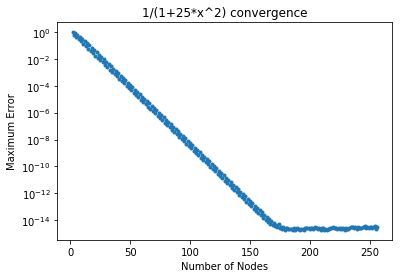
\includegraphics[width=0.8\textwidth]{q2diia.png}
            \caption{Convergence of $f(x) = \frac{1}{1+25x^2}$}
          \end{figure}

          \begin{figure}[H]
            \centering
              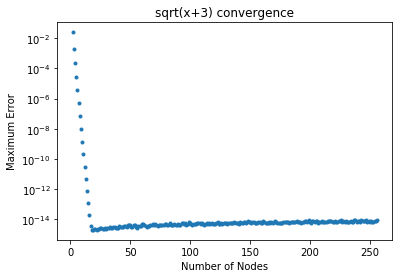
\includegraphics[width=0.8\textwidth]{q2diib.png}
            \caption{Convergence of $f(x) = \sqrt{x+3}$}
          \end{figure}

          \begin{figure}[H]
            \centering
              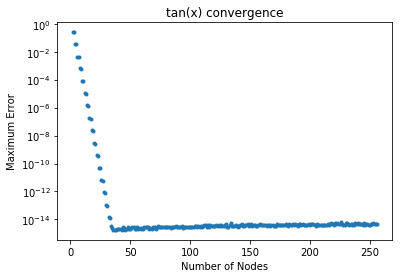
\includegraphics[width=0.8\textwidth]{q2diic.png}
            \caption{Convergence of $f(x) = \tan x$}
          \end{figure}

        \item See the plots below. The slopes do appear to curve increasingly steep before rounding errors occur for the first two functions. For the last function, $f(x) = \cos(100 \pi x)$, the number of zeroes in $[-1,1]$ are so great that even for $N=256$, there are not enough points to interpolate accurately.
          \begin{figure}[H]
            \centering
              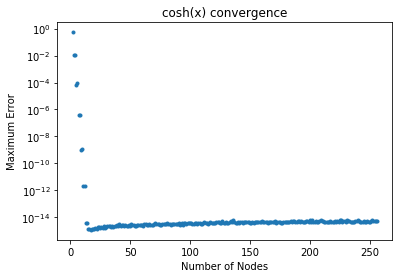
\includegraphics[width=0.8\textwidth]{q2diiia.png}
            \caption{Convergence of $f(x) = \cosh x$}
          \end{figure}

          \begin{figure}[H]
            \centering
              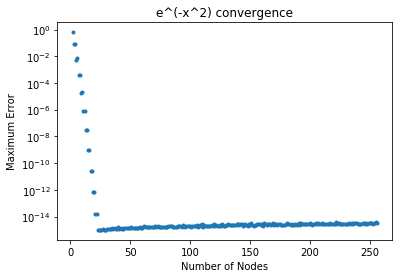
\includegraphics[width=0.8\textwidth]{q2diiib.png}
            \caption{Convergence of $f(x) = e^{-x^2}$}
          \end{figure}

          \begin{figure}[H]
            \centering
              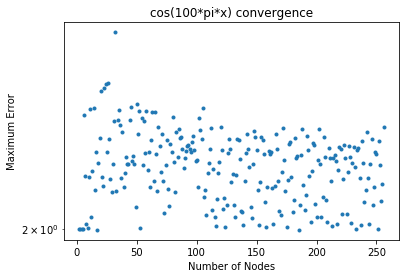
\includegraphics[width=0.8\textwidth]{q2diiic.png}
            \caption{Convergence of $f(x) = \cos(100 \pi x)$}
          \end{figure}

      \end{enumerate}

  \end{enumerate}
\end{answer}

\begin{exercise}
  \textbf{Chebyshev coefficients via the DCT}
\end{exercise}

\begin{answer}
  \begin{enumerate}[label=\alph*)]

    \item See the implementation in \texttt{question3.ipynb}

    \item
      \begin{enumerate}[label=\roman*)]
        \item By inspection, the following Chebyshev polynomials satisfy the equation
          \begin{gather*}
            f(x) = T_4(x) + T_3(x) + 5 T_2(x) + 4 T_1(x) + 5 T_0(x)
          \end{gather*}

        \item See the implementation in \texttt{question3.ipynb}. It matches the above.
      \end{enumerate}

    \item The running times are in the table below. See the implementation in \texttt{question3.ipynb}.
      \begin{center}
        \begin{tabular}{ c | c }
          Nodes & Time \\
          \hline
          $2^{10}$ & 330.6 $\mu$s \\
          $2^{13}$ & 61.03 ms \\
          $2^{13}$+1 & 520.0 $\mu$s \\
          $2^{17}$ & 14.91 s \\
          $2^{17}$+1 & 5.792 ms \\
        \end{tabular}
      \end{center}

      The plot below shows the computation time for different number of nodes. Notice that the computation time rises somewhere between $O(k)$ (orange line) and $O(k^2)$ (green line).
      \begin{figure}[H]
        \centering
          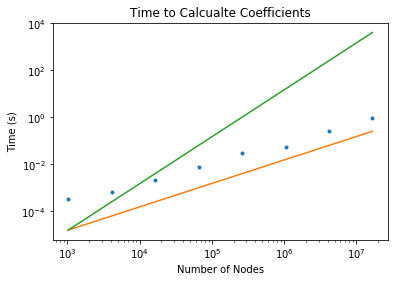
\includegraphics[width=0.8\textwidth]{q3c.png}
        \caption{Computation Time vs. Number of Nodes}
      \end{figure}
  \end{enumerate}
\end{answer}

\end{document}